\section{Лекция 10 12.05.24}

Одномерное стационарное уравнение теплопроводности:
\[
(p(x)y')' - q(x)y = -f(x), \quad 0 < x < \ell,
\]
где:
\begin{itemize}
  \item \( p(x) \in C^1[0,\ell] \) — заданная функция теплопроводности среды. Полагаем, что существует\( c > 0 \), такое что \( p(x) \ge c \quad \forall x \in [0,\ell] \);

  \item \( q(x) \in C[0,\ell] \), \( q(x) \ge 0 \) — заданная функция поглощение тепла (например, теплопотери в среде);

  \item \( f(x) \in C[0,\ell] \) — заданная непрерывная функция, описывающая плотность распределённых источников тепла;

  \item \( y(x) \) — неизвестная функция, которую требуется найти. Она интерпретируется как распределение температуры по телу.
\end{itemize}


\paragraph{Краевая задача первого рода}
\[
\begin{cases}
(p(x)y')' - q(x)y = -f(x), & 0 < x < \ell, \\
y(0) = \mu_0, \\
y(\ell) = \mu_\ell.
\end{cases}
\]
Так же введём 2 нормы:
\[
\|u\|_C := \max_{x \in [0,\ell]} |u(x)|, \quad \|u\|_{C^1} := \max_{x \in [0,\ell]} \left( |u(x)| + |u'(x)| \right).
\]

\paragraph{Переход к однородным краевым условиям.} Рассмотрим краевую задачу:
\[
\begin{cases}
(p(x) y')' - q(x) y = -f(x), & 0 < x < \ell, \\
y(0) = \mu_0, \\
y(\ell) = \mu_\ell.
\end{cases}
\]
Введём вспомогательную функцию:
\[
v(x) = \mu_0 + \frac{x}{\ell}(\mu_\ell - \mu_0),
\]
которая удовлетворяет граничным условиям:
\[
v(0) = \mu_0, \quad v(\ell) = \mu_\ell.
\]
Тогда можно показать, что:
\[
(p(x) v')' - q(x) v = \frac{\mu_\ell - \mu_0}{\ell} p'(x) - q(x)\left(\mu_0 + \frac{x}{\ell}(\mu_\ell - \mu_0)\right).
\]
Подставим \( y = v + z \). Тогда $z$ удовлетворяет уравнению:
\[
\begin{cases}
(p(x) z')' - q(x) z = -f(x) - \dfrac{\mu_\ell - \mu_0}{\ell} p'(x) + q(x) v(x), & 0 < x < \ell, \\
z(0) = 0, \\
z(\ell) = 0.
\end{cases}
\]
Таким образом, далее будет рассматриать только задачу с однородными граничными условиями.


\subsection{Функциональный вид задачи теплопроводности}

Рассмотрим следующий оператор:
\[
A u(x) = -\big(p(x) u'(x)\big)' + q(x) u(x), \quad x \in (0, \ell).
\]
Область определения оператора:
\[
\mathfrak{D}_A = \left\{ u \in C^2[0,\ell] \ \middle|\ u(0) = u(\ell) = 0 \right\}.
\]
Таким образом, оператор $A$ действует на дважды непрерывно дифференцируемые функции, обращающиеся в ноль на концах отрезка.

\subsubsection{Пространство $L^2(0,\ell)$ и его свойства}
Пространство $L^2(0,\ell)$ состоит из измеримых функций $f$, удовлетворяющих:
\[
\int_0^\ell f^2(x) \, dx < +\infty.
\]
Скалярное произведение:
\[
(u, v) = \int_0^\ell u(x) v(x) \, dx, \quad \|u\|_{L^2} = \sqrt{(u, u)}= \left( \int_0^\ell u^2(x) \, dx \right)^{1/2}.
\]
Известные факты:
\begin{itemize}
  \item $L^2(0,\ell)$ — гильбертово пространство, т.е. полное по мере поражденной скалярным произведением.
  \item Неравенство Коши--Буняковского:
  \[
  |(u, v)| \leq \|u\|_{L^2} \cdot \|v\|_{L^2}.
  \]
  \[
  | \int_0^\ell u(x) v(x) \, dx | \le \left( \int_0^\ell u^2(x) \, dx \right)^{1/2} \left( \int_0^\ell v^2(x) \, dx \right)^{1/2}
  \]
  \item Пусть $f \in L^2[a,b]$. Рассмотрим скалярное произведение функции $f$ с тождественно единичной функцией $g(x) \equiv 1$:
    \[
    \left( \int_a^b f(x) \, dx \right)^2 = \left( \int_a^b f(x) \cdot 1 \, dx \right)^2.
    \]
    Применим неравенство Коши--Буняковского:
    \[
    \left( \int_a^b f(x) \cdot 1 \, dx \right)^2 \le \left( \int_a^b f^2(x) \, dx \right) \left( \int_a^b 1^2 \, dx \right).
    \]
    Так как $\int_a^b 1 \, dx = b - a$, получаем:
    \[
    \left( \int_a^b f(x) \, dx \right)^2 \le (b - a) \int_a^b f^2(x) \, dx.
    \]
\end{itemize}

\subsubsection{Классическое решение задачи}

\paragraph{Определение.} Если $f \in L^2(0,\ell)$ и существует функция $y_0 \in \mathfrak{D}_A$ такая, что:
\[
A y_0 = f,
\]
то $y_0$ называется \textit{классическим решением} задачи.

\paragraph{Пример.}
\[
f(x) =
\begin{cases}
1, & 0 \leq x \leq \frac{\ell}{2}, \\
-1, & \frac{\ell}{2} < x \leq \ell.
\end{cases}
\]
Тогда $f \in L^2(0,\ell)$, однако уравнение $A y = f$ не имеет классического решения.

\subsubsection{Свойства оператора}

\paragraph{Симметричность.} Для $u, v \in \mathfrak{D}_A$ рассмотрим скалярное произведение:
\[
(A u, v) = \int_0^\ell \left[-(p(x) u'(x))' + q(x) u(x)\right] v(x) \, dx.
\]
Интегрируя первую часть по частям:
\[
\int_0^\ell -(p u')' v \, dx = \left[-p u' v \right]_0^\ell + \int_0^\ell p u' v' \, dx.
\]
Так как $v(0) = v(\ell) = 0$, то граничные члены зануляются. Получаем:
\[
(A u, v) = \int_0^\ell \left[ p(x) u'(x) v'(x) + q(x) u(x) v(x) \right] \, dx.
\]
Аналогично получим, что:
\[
(u, A v) = \int_0^\ell \left[ p(x) u'(x) v'(x) + q(x) u(x) v(x) \right] \, dx.
\]
Следовательно, $(A u, v) = (u, A v)$, и оператор $A$ симметричен на $ \mathfrak{D}_A $.

\paragraph{Положительная определённость.} Положительная определённость:
\[
(A u, u) = \int_0^\ell \left[ p(x) (u'(x))^2 + q(x) u^2(x) \right] \, dx.
\]
Так как $p(x) \ge c > 0$, $q(x) \ge 0$, получаем:
\[
(A u, u) \ge c \int_0^\ell (u')^2 \, dx.
\]
Таким образом, оператор $A$ положительно определён на $\mathfrak{D}_A$.

\paragraph{Лемма об оценке норм.} Для $u \in C^1[0,\ell]$, $u(0) = u(\ell) = 0$ выполнены оценки:
\[
\|u\|_{L^2} \le \frac{\ell}{2} \|u'\|_{L^2}, \quad \|u\|_C \le \frac{\sqrt{2} \, \ell}{2} \|u'\|_{L^2}.
\]
\textbf{Доказательство.} Из формулы Ньютона--Лейбница:
\[
u(x) = \int_0^x u'(\beta) \, d\beta = -\int_x^\ell u'(\beta) \, d\beta.
\]
Тогда:
\[
\ell u^2(x) = (\ell - x) u^2(x) + x u^2(x) =
(\ell - x) \left[ \int_0^x u'(\beta) \, d\beta \right]^2 + x \left[ \int_x^\ell u'(\beta) \, d\beta \right]^2
= (*)
\]
Применяя неравенство Коши--Буняковского:
\[
\ell u^2(x) \le (\ell - x) x \int_x^\ell u'^2(\beta) \, d\beta + x (\ell - x) \int_0^x u'^2(\beta) \, d\beta = (\ell - x) x \int_x^\ell u'^2(\beta) \, d\beta \le \frac{\ell^2}{4} \|u'\|_{L^2}
\]
Следовательно:
\[
    \|u\|_C \le \frac{\sqrt{\ell}}{2} \|u'\|_{L^2}
\]
\[
    \|u\|_{L^2} = \left( \int_0^\ell u^2(x) \, dx \right)^{1/2} \le \|u\|_c \left( \int_0^\ell dx \right)^{1/2} = \sqrt{l} \|u\|_C \le \frac{l}{2} \|u'\|_{L^2}
\]

\paragraph{Энергетическая норма.} Так как оператор симметричен и положительно определён, то а пространстве $ \mathfrak{D}_A $ можем ввести энергетическое скалярное произведение:
\[
(u, v)_A = \int_0^\ell \left[ p(x) u'(x) v'(x) + q(x) u(x) v(x) \right] \, dx,
\]
и соответствущую норму:
\[
\|u\|_A = \sqrt{(u, u)_A}.
\]

\paragraph{Замечание.} Рассмотрим последовательность функций:
\[
u_n(x) =
\begin{cases}
x, & 0 \le x \le \frac{\ell}{2} - \frac{1}{n}, \\
a_n + b_n(x - \frac{\ell}{2}) + c_n(x - \frac{\ell}{2})^2, & \frac{\ell}{2} - \frac{1}{n} < x < \frac{\ell}{2}, \\
\ell - x, & \frac{\ell}{2} \le x \le \ell.
\end{cases}
\]
Параметры $a_n$, $b_n$, $c_n$ подбираются так, чтобы $u_n \in \mathfrak{D}_A$ (гладкость и граничные условия выполнены).
Можно показать, что:
\[
\|u_n - u\|_A \xrightarrow[n \to \infty]{} 0, \quad \text{где } u(x) = \min(x, \ell - x).
\]
Однако $u(x) \notin \mathfrak{D}_A$ (из-за негладкости в точке $x = \ell/2$).
Следовательно, пространство $\mathfrak{D}_A$ не является полным в энергетической норме. Определим  $H_A$ как пополнение $\mathfrak{D}_A$ всеми пределами всех функциональных последовательностей по энергетичекой норме.

\paragraph{Факт.} $H_A$ — бесконечномерное сепарабельное гильбертово пространство. Этот факт доказывается через теорию пространств Соболева.

\subsubsection{Обобщённое решение}

\paragraph{Теорема (Рисса).}
Пусть $H$ — гильбертово пространство, а $F: H \to \mathbb{R}$ — линейный непрерывный ограниченный функционал. Тогда существует единственный элемент $u \in H$, такой что:
\[
F(v) = (u, v)_H, \quad \forall v \in H.
\]

\paragraph{Определение.}
Функция $y \in H_A$ называется \textit{обобщённым решением} краевой задачи, если для любого $v \in H_A$ выполнено:
\[
\int_0^\ell \left[ p(x) y'(x) v'(x) + q(x) y(x) v(x) \right] dx = \int_0^\ell f(x) v(x) dx.
\]

\paragraph{Теорема.}
Пусть $f \in L^2(0,\ell)$. Тогда обобщенное решение существует и единственно.
\textbf{Доказательство.}
Рассмотрим линейный функционал:
\[
F(v) := \int_0^\ell f(x) v(x) \, dx.
\]
Этот функционал корректно определён на $H_A$, поскольку $f \in L^2(0,\ell)$ и $H_A \subset L^2(0,\ell)$. Линейность очевидна.
Проверим ограниченность \( F \) в норме \( \|\cdot\|_A \). По неравенству Коши--Буняковского:
\[
|F(v)| \le \|f\|_{L^2} \cdot \|v\|_{L^2}.
\]
Оценим \( \|v\|_{L^2} \) через \( \|v\|_A \). Из ранее доказанной оценки (леммы):
\[
\|v\|_{L^2} \le \frac{\ell}{2} \|v'\|_{L^2}.
\]
С другой стороны, из определения энергетической нормы:
\[
\|v\|_A^2 = \int_0^\ell \left[ p(x)(v')^2 + q(x)v^2 \right] dx \ge c \int_0^\ell (v')^2 dx = c \|v'\|_{L^2}^2,
\]
где \(с\) -- константа из определения \(p(x)\).
Отсюда:
\[
\|v'\|_{L^2} \le \frac{1}{\sqrt{c}} \|v\|_A,
\quad \text{а значит} \quad
\|v\|_{L^2} \le \frac{\ell}{2} \cdot \frac{1}{\sqrt{c}} \|v\|_A = \frac{\ell}{2\sqrt{c}} \|v\|_A.
\]
Итак:
\[
|F(v)| \le \|f\|_{L^2} \cdot \|v\|_{L^2} \le \|f\|_{L^2} \cdot \frac{\ell}{2\sqrt{c}} \cdot \|v\|_A.
\]
Следовательно, \( F \) — ограниченный функционал на гильбертовом пространстве \( H_A \).
По теореме Рисса существует и единственен элемент \( y \in H_A \), такой что:
\[
F(v) = (y, v)_A, \quad \forall v \in H_A.
\]
Что и означает, что \( y \) является обобщённым решением задачи. \hfill $\square$

\paragraph{Замечания.}
\begin{enumerate}
  \item Если обобщённое решение $y \in H_A$ принадлежит также $\mathfrak{D}_A$, то оно является классическим решением.
  \item Если классическое решение существует, то оно автоматически является обобщённым.
\end{enumerate}

\subsection{Метод Галёркина}
Пока мы только поставили задачу в функциональном виде, но ничего не сказали о её численном решении.
\paragraph{Факт.} В любом сепарабельном гильбертовом пространстве существует счётный ортонормированный базис. Поэтому:
\begin{itemize}
  \item Существует базис $\{\varphi_j\}_{j=1}^\infty$ в $H_A$.
  \item Обозначим $W_N := \mathrm{span}\{\varphi_1, \dots, \varphi_N\} \subset H_A$.
  \item Тогда любой $u \in W_N$ имеет представление:
  \[
  u(x) = \sum_{j=1}^N u_j \varphi_j(x), \quad u_j \in \mathbb{R}.
  \]
\end{itemize}

\subsubsection{Приближённое решение}
\paragraph{Определение.} Приближённым обобщённым решением называется функция $y_N \in W_N$, такая что:
\[
(y_N, v)_A = (f, v), \quad \forall v \in W_N.
\]

\paragraph{Теорема.} Для любого $f \in L^2(0,\ell)$ и любого $N \in \mathbb{N}$ приближённое обобщённое решение $y_N \in W_N$ существует и единственно.

\textbf{Доказательство.}

Берём доказательство теоремы о существовании обобщённого решения и заменяем всё пространство $H_A$ на конечномерное $W_N$. Поскольку $W_N$ — подпространство гильбертова пространства, всё рассуждение сохраняется.
\hfill $\square$

Вместо поиска $y \in H_A$ ищем последовательность приближённых решений $y_N \in W_N$. Нужно только обеспечить сходимость этих приближений.
\textit{Это и есть суть метода Галёркина.}

\subsubsection{Борис Григорьевич Галёркин и Даниил Андреев}

\begin{center}
	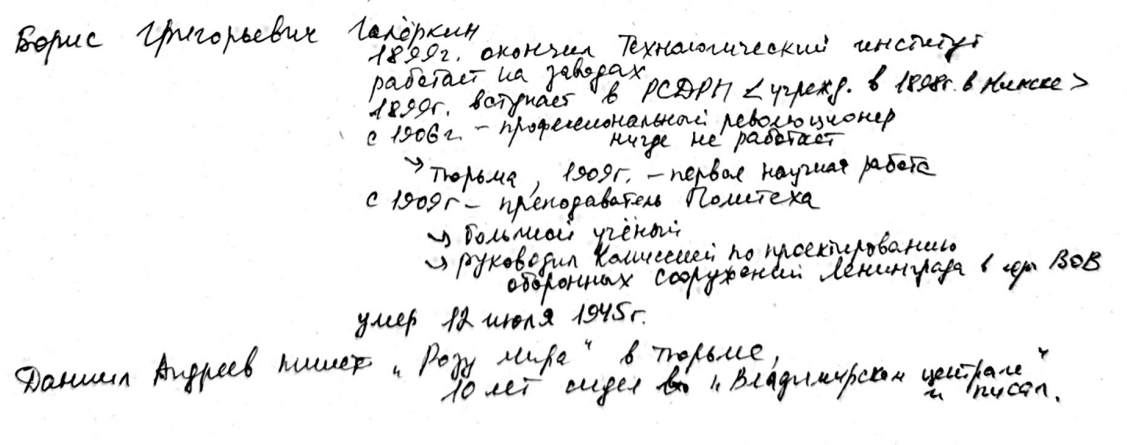
\includegraphics[width=18cm]{../figures/lection_10/figure_1.png}
\end{center}

\subsubsection{Вывод системы уравнений}
Пусть:
\[
y_N(x) = \sum_{j=1}^N y_j \varphi_j(x).
\]
Тогда потребуем, чтобы:
\[
(y_N, \varphi_k)_A = (f, \varphi_k), \quad k = 1, \dots, N.
\]
Подставим:
\[
\left( \sum_{j=1}^N y_j \varphi_j, \varphi_k \right)_A = \sum_{j=1}^N y_j (\varphi_j, \varphi_k)_A.
\]
Получаем СЛАУ:
\[
\sum_{j=1}^N A_{kj} y_j = b_k, \quad \text{где } A_{kj} = (\varphi_j, \varphi_k)_A, \quad b_k = (f, \varphi_k).
\]
Матрица $A = (A_{kj})$ — это матрица Грама в энергетическом скалярном произведении. Она симметрична и положительно определена, значит — невырождена. А что на счёт сходимости?

\paragraph{Лемма (об ортогональности).}
Приближённое обобщённое решение $y_N \in W_N$ является ортогональной проекцией точного решения $y \in H_A$ на подпространство $W_N$:
\[
\forall u \in W_N \quad (y_N - y, u)_A = 0.
\]
\textbf{Доказательство.}
По определению обобщённого решения:
\[
(y, u)_A = (f, u), \quad \forall u \in H_A.
\]
По определению приближённого обобщённого решения:
\[
(y_N, u)_A = (f, u), \quad \forall u \in W_N.
\]
Значит:
\[
(y_N - y, u)_A = 0, \quad \forall u \in W_N.
\]
\hfill $\square$

\paragraph{Вывод.}
Фактически, метод Галёркина ищет проекцию точного решения $y$ на конечномерное подпространство $W_N$ в энергетической норме. В этом смысле метод является проекционным.

\paragraph{Лемма (о наилучшем приближении).}
Приближённое решение $y_N$ минимизирует расстояние до $y$ в энергетической норме:
\[
\|y - y_N\|_A = \inf_{u \in W_N} \|y - u\|_A.
\]
\textbf{Доказательство.}
Пусть $u \in W_N$. Тогда $y_N - u \in W_N$, и, по лемме об ортогональности:
\[
(y_N - y, y_N - u)_A = 0.
\]
Рассмотрим:
\[
\|y - u\|_A^2 = \|y - y_N + y_N - u\|_A^2 = \|y - y_N\|_A^2 + \|y_N - u\|_A^2.
\]
Отсюда:
\[
\|y - y_N\|_A^2 \le \|y - u\|_A^2, \quad \forall u \in W_N.
\]
Минимум достигается при $u = y_N$. \hfill $\square$

\paragraph{Неформальный вывод.}

Если базис $\{\varphi_j\}$ "хорошо приближает" всё пространство $H_A$ (в смысле предельной плотности), то:
\[
\|y - y_N\|_A \to 0,
\]
а значит, приближённые обобщённые решения $y_N$ стремятся к точному решению $y$ — не только формально, но и конструктивно.

\paragraph{Определение.}
Бесконечная последовательность вложенных подпространств $W_N \subset H_A$ называется \textit{предельно плотной} в $H_A$, если:
\[
\forall \varepsilon > 0, \ \forall y \in H_A \ \exists N_0: \ \forall N > N_0 \quad \inf_{u \in W_N} \|y - u\|_A < \varepsilon.
\]

\paragraph{Теорема.}
Если $\{W_N\}$ предельно плотна в $H_A$, то приближения $y_N \in W_N$, построенные по методу Галёркина, сходятся к точному обобщённому решению $y \in H_A$:
\[
\|y_N - y\|_A \to 0, \quad \text{при } N \to \infty.
\]
Более того, имеет место и сходимость в $L^2(0,\ell)$:
\[
\|y_N - y\|_{L^2} \le \frac{\ell}{2\sqrt{c}} \|y_N - y\|_A,
\]
\textbf{Доказательство.}
Пусть $y \in H_A$ — обобщённое решение, и $\varepsilon > 0$ — произвольное. По определению предельной плотности, существует $N_0$, такое что:
\[
\forall N > N_0 \quad \exists u \in W_N: \ \|y - u\|_A < \varepsilon.
\]
Из леммы о наилучшем приближении:
\[
\|y - y_N\|_A \le \inf_{u \in W_N} \|y - u\|_A < \varepsilon.
\]
Отсюда:
\[
\|y - y_N\|_{L^2} \le \frac{\ell}{2\sqrt{c}} \|y - y_N\|_A < \frac{\ell}{2\sqrt{c}} \varepsilon.
\]
\hfill $\square$

\subsubsection{Построение базиса}
Как построить базис в пространстве $H_A$? Универсального рецепта нет, но можно привести пример.

\paragraph{Пример.}
\[
p(x) \equiv 1, \quad q(x) \equiv 0,
\]
тогда оператор:
\[
A u(x) = -u''(x), \quad u \in \mathfrak{D}_A, \quad x \in (0,\ell).
\]
Рассмотрим собственные функции задачи:
\[
\varphi_k(x) = \sqrt{\frac{2}{\ell}} \sin\left( \frac{k \pi x}{\ell} \right), \quad k = 1, 2, \dots
\]
Тогда:
\begin{itemize}
  \item $\{\varphi_k\}$ — ортонормированная система в $L^2(0,\ell)$;
  \item функции $\varphi_k$ принадлежат $H_A$;
  \item система полная в $L^2(0,\ell)$, а значит — и в $H_A$ (с замыканием).
\end{itemize}
Любую функцию $u \in H_A$ можно представить в виде:
\[
u(x) = \sum_{k=1}^\infty \mu_k \varphi_k(x), \quad \mu_k = (u, \varphi_k)_{L^2}, \quad \text{сходимость в } H_A.
\]
Таким образом, $\{\varphi_k\}$ — базис в $H_A$, а приближение в $W_N := \mathrm{span}\{\varphi_1, \dots, \varphi_N\}$ имеет вид:
\[
y_N(x) = \sum_{j=1}^N y_j \varphi_j(x),
\]
где $y_j$ определяются из системы Галёркина:
\[
\sum_{j=1}^N ( \varphi_j, \varphi_k )_A y_j = (f, \varphi_k), \quad k = 1, \dots, N.
\]

\subsubsection{Проблемы классического метода Галёркина}
\begin{itemize}
  \item Непонятно, откуда брать базис $\{\varphi_j\}$ для произвольного оператора $A$;
  \item Матрица СЛАУ часто получается плотной (все элементы ненулевые);
\end{itemize}
Чтобы решить эти проблемы рассмотрим \textbf{метод конечных элементов (МКЭ)} — это частный случай метода Галёркина, в котором используются \emph{особые} базисные функции.

\subsection{Метод конечных элементов (МКЭ)}
Для определения базисных функций в МКЭ требуется ввести сетку. Поэтому метод конечных элементов — \textit{проекционно-сеточный метод}.

Рассмотрим равномерную сетку \( \tilde{\Pi}_h \) на отрезке \( [0,1] \) с шагом \( h \).
А так же рассмотрим \( x: z \in [1, 0] \to x(z)  \) — строго возрастающее преобразование, такое что:
\[
x(0) = 0, \quad x(1) = \ell, \quad 0 < l_1 \le \frac{dx}{dz} \le l_2 < +\infty.
\]
Определим сетку \( \Pi_h \) на отрезке \( [0, \ell] \) как образ узлов \( \tilde{\Pi}_h \) при отображении \(x(z)\):
\[
x_j := x(z_j), \quad j = 0, 1, \dots, N.
\]
Обозначим:
\[
h_{j+1/2} := x_{j+1} - x_j, \qquad h_{\max} := \max_j h_{j+1/2}.
\]
Можно показать \( h_{\max} \xrightarrow[h \to 0]{} 0 \).

\paragraph{Базисные функции.} Введём следующие кусочно-линейные функции:
\[
\varphi_j(x) =
\begin{cases}
\dfrac{x - x_{j-1}}{h_j}, & x_{j-1} \le x \le x_j, \\
\dfrac{x_{j+1} - x}{h_{j+1}}, & x_j \le x \le x_{j+1}, \\
0, & \text{иначе},
\end{cases}
\quad j = 1, \dots, N-1.
\]
Также определим крайние функции (при необходимости):
\[
\varphi_0(x) =
\begin{cases}
\dfrac{x_1 - x}{h_1}, & 0 \le x \le x_1, \\
0, & \text{иначе},
\end{cases}
\qquad
\varphi_N(x) =
\begin{cases}
\dfrac{x - x_{N-1}}{h_N}, & x_{N-1} \le x \le \ell, \\
0, & \text{иначе}.
\end{cases}
\]
Но если \( y(0) = y(\ell) = 0 \), то в базис входят только \( \varphi_1, \dots, \varphi_{N-1} \).

\paragraph{Свойства базисных функций:}

\begin{itemize}
  \item \( \varphi_j(x_k) = \delta_{jk} \);
  \item \( \{ \varphi_j \}_{j=1}^{N-1} \) — линейно независимы;
  \item имеют компактный носитель: \( \mathrm{supp}(\varphi_j) \subset [x_{j-1}, x_{j+1}] \);
  \item \( \varphi_j \in H_A \), т.е. удовлетворяют граничным условиям и гладкости внутри отрезка.
\end{itemize}
\textbf{Следствие:} \( \{ \varphi_j \}_{j=1}^{N-1} \) образуют базис в пространстве \( W_h \subset H_A \):
\[
W_h := \mathrm{span}\{ \varphi_1, \dots, \varphi_{N-1} \}.
\]
Рассмотрим пространство
\[
W_{n-1} := \mathrm{span}\{\varphi_1, \dots, \varphi_{n-1}\},
\]
Каждая функция \( u \in W_h \) имеет вид:
\[
u(x) = \sum_{j=1}^{N-1} c_j \varphi_j(x), \quad c_j = u(x_j).
\]
В частности,
\[
y_N(x) = \sum_{j=1}^{N-1} y_j \varphi_j(x),
\]
где \( y_j = y_h(x_j) \).
Но учитывая локальность носителей, получим:
\[
(\varphi_{j-1}, \varphi_j)_A y_{j-1} + (\varphi_j, \varphi_j)_A y_j + (\varphi_{j+1}, \varphi_j)_A y_{j+1} = (f, \varphi_j), \quad j = 1, \dots, N-1.
\]
Граничные условия: \( y_0 = 0, \quad y_N = 0 \).
И мы получаем систему с трёхдиагональной матрицей:
\[
(\varphi_j, \varphi_j)_A = \frac{1}{h_{j+1/2}^2} \int_{x_{j-1}}^{x_{j+1}} \left[ -p(x) + q(x)(x - x_{j - 1})(x_j - x) \right] dx.
\]
Система может быть решена методом прогонки при выполнении условия:
\[
h_{\max} \le \sqrt{\frac{6 c}{Q}}, \quad Q = \max_{x \in [0, \ell]} q(x).
\]

\paragraph{Теорема.} Приближённое решение \( y_h(x) \), полученное с помощью МКЭ, при \( h \to 0 \) сходится в \( H_A \) к точному обобщённому решению задачи. Более точно:
\[
\| y_h - y \|_{L^2} \le c h^2 \|f\|_{L^2},
\]

\paragraph{Замечание.} Можно рассматривать и более сложные базисные функции (например, кусочно-квадратичные) и получать более точные приближения.